\documentclass[12pt,a4paper,openright,final]{article}
\usepackage{fontspec}
\usepackage{amsmath}
\usepackage{amsfonts}
\usepackage{amssymb}
\usepackage{makeidx}
\usepackage{graphicx}
\usepackage[hidelinks,unicode=true]{hyperref}
\usepackage[spanish,es-nodecimaldot,es-lcroman,es-tabla,es-noshorthands]{babel}
\usepackage[left=3cm,right=2cm, bottom=4cm]{geometry}
\usepackage{natbib}
\usepackage{microtype}
\usepackage{ifdraft}
\usepackage{verbatim}
\usepackage[obeyDraft]{todonotes}
\ifdraft{
	\usepackage{draftwatermark}
	\SetWatermarkText{BORRADOR}
	\SetWatermarkScale{0.7}
	\SetWatermarkColor{red}
}{}
\usepackage{booktabs}
\usepackage{longtable}
\usepackage{calc}
\usepackage{array}
\usepackage{caption}
\usepackage{subfigure}
\usepackage{footnote}
\usepackage{url}
\usepackage{tikz}

\setsansfont[Ligatures=TeX]{texgyreadventor}
\setmainfont[Ligatures=TeX]{texgyrepagella}

\author{José Ignacio Escribano}

\title{Actividad II. Ingeniería de la Decisión \\ \textbf{Resolución de un problema de decisión con GeNIe}}

\setlength{\parindent}{0pt}

\begin{document}

\maketitle

\textbf{Enunciado:} Se le presenta la oportunidad de adquirir una opción del Gobierno cubano para explotar un pozo de petróleo de 5.000.000 de barriles a 5 € por barril. Repsol cree que después de procesamiento, transporte y refino, puede obtener 8 € por barril en el mercado USA. Sin embargo, a consecuencia de la ley Helms-Burton, Repsol teme no recibir autorización del gobierno USA, con lo que debería pagar una multa a Cuba de 1€ por barril, por no hacer efectiva la operación. Repsol estima que hay probabilidad 0.7 de no recibir la autorización para la importación si gana el Partido Republicano en el Congreso  y 0.4 si gana el Partido Demócrata. En estos momentos, NYT da ganador al Partido Republicano con probabilidad 0.56.\\

Para reducir su incertidumbre, estudia contratar a Arnald’s, un bufete que puede estudiar en detalle el caso por 100.000 €, y puede hacer un informe ``Favorable'' o ``Desfavorable''. Según el dossier que presenta Arnald’s, de 20 ocasiones previas que se consiguió la autorización, en 19 emitió informe ``Favorable''. Igualmente, indican que en 10 ocasiones en que no se recibió la autorización, habían emitido informe favorable en 3 de ellas.\\
 
Determinar si merece o no la pena contratar a Arnald’s, y si Repsol debe ejercer o no la opción, resolviendo el  diagrama de influencia del problema con GeNIe.\\

¿Cambia la solución si la probabilidad de que gane el Partido Republicano  es 0.4? ¿Y si fuese 0.8?\\

\textbf{Solución:} En primer lugar, identificamos los objetivos, incertidumbres del problema y las decisiones que debe tomar Repsol.\\

El objetivo es maximizar el beneficio. Las incertidumbres son el ganador de las elecciones según la encuesta del New York Times, recibir la autorización y el resultado del informe. Las decisiones que debe tomar Repsol son explotar o no el pozo y contratar o no al bufete de abogados Arnald's.\\

El diagrama de influencia completo se muestra en la Figura~\ref{fig:diagrama_influencia}. Los estados de cada incertidumbre y las elecciones de las decisiones se muestran a continuación:

\begin{figure}[tbph!]
	\centering
	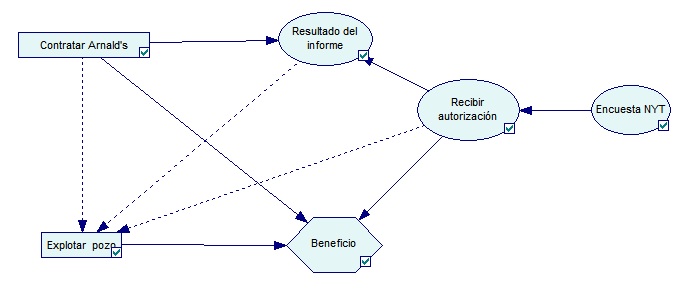
\includegraphics[width=\linewidth]{imagenes/diagrama_influencia.png}
	\caption{Diagrama de influencia del problema}
	\label{fig:diagrama_influencia}
\end{figure}

\begin{itemize}
	\item Contratar Arnald's:
	
	\begin{itemize}
		\item Contratar
		\item No contratar
	\end{itemize}
	
	\item Explotar pozo:
	
	\begin{itemize}
		\item Explotar
		\item No explotar
	\end{itemize}
	
	\item Resultado del informe
	
	\begin{itemize}
		\item Favorable
		\item Desfavorable
		\item No hacer (si no se contrata a Arnald's)
	\end{itemize} 
	
	\item Recibir autorización
	
	\begin{itemize}
		\item Recibir
		\item No recibir
	\end{itemize}
	
	\item Encuesta NYT
	
	\begin{itemize}
		\item Partido Republicano
		\item Partido Demócrata
	\end{itemize}
	
\end{itemize}

Teniendo en cuenta los datos del enunciado se introducen las probabilidades de los nodos de azar en GeNIe, que se muestran en la Figura~\ref{fig:azar}.

\begin{figure}[htbp!]
	\centering
	\subfigure[Probabilidades del nodo Encuesta NYT]{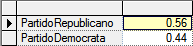
\includegraphics[width=0.45\linewidth]{./imagenes/nyt}}\hspace{10mm}
	\subfigure[Probabilidades del nodo Recibir autorización]{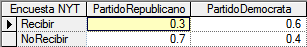
\includegraphics[width=0.45\linewidth]{./imagenes/autorizacion}}\vspace{10mm}
	\subfigure[Probabilidades del nodo Resultado informe]{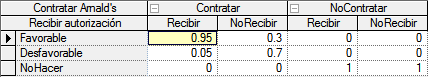
\includegraphics[width=0.9\linewidth]{./imagenes/resultado_informe}}
	\caption{Probabilidades de los nodos de azar} \label{fig:azar}
\end{figure}

Sólo nos queda introducir la utilidad del nodo Beneficio. Para ello, calculamos el beneficio (en millones de euros) de cada una de las posibilidades (Figura~\ref{fig:utilidad}).\\

\begin{figure}[tbph!]
	\centering
	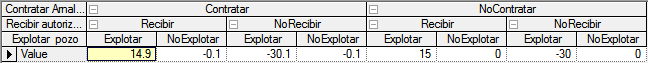
\includegraphics[width=\linewidth]{imagenes/utilidad.png}
	\caption{Utilidad del nodo Beneficio}
	\label{fig:utilidad}
\end{figure}

Consideremos algún ejemplo. La utilidad de explotar el pozo, sabiendo que hemos recibido la autorización y hemos contratado a Arnald's es -0.1 (por contratar a Arnald's) -5*5 (por explotar el pozo) + 8*5 (por vender en el mercado USA) = 14.9 millones de euros.\\

La utilidad de explotar el pozo sabiendo que no hemos recibido la autorización y habiendo contratado a Arnald's es -0.1 (por contratar a Arnald's) -5*5 (por explotar el pozo) - 1*5 (multa de Cuba por no tener la autorización) = -30.1 millones de euros.\\

De forma similar se obtiene el resto de los casos.\\

Sólo nos queda calcular el modelo con GeNIE para obtener los resultados. Los resultados (Figura~\ref{fig:resultado}) que se obtienen son los siguientes:\\

\begin{figure}[tbph!]
	\centering
	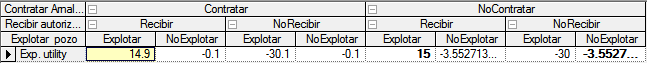
\includegraphics[width=\linewidth]{imagenes/resultado.png}
	\caption{Resultados del modelo}
	\label{fig:resultado}
\end{figure}

Observamos que el la máxima utilidad esperada se obtiene cuando se decide no contratar a Arnald's, se recibe la autorización y se explota el pozo.\\

Si observamos los resultados del nodo Contratar Arnald's, la utilidad de Contratar es 6.38 y 6.48 para NoContratar. Por lo que no debemos contratar a este bufete de abogados.\\

Si ahora observamos los resultados del nodo Explotar pozo, observamos que tanto si contratamos como si no contratamos a Arnald's, la mejor opción es explotar el pozo si recibimos la autorización, y no explotar en caso de no recibirla, aunque el de máxima utilidad será cuando no se le contrate.\\

\begin{figure}[tbph!]
	\centering
	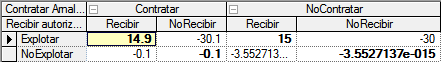
\includegraphics[width=\linewidth]{imagenes/resultados_pozo.png}
	\caption{Resultados del nodo Explotar pozo}
	\label{fig:resultados_pozo}
\end{figure}

En definitiva, para obtener la máxima utilidad, deberemos no contratar al bufete de abogados Arnald's, y explotar el pozo en caso de obtener la autorización, y no explotar si no obtenemos la autorización.\\

Si ahora la probabilidad de que gane el partido Republicano es de 0.4, debemos cambiar las probabilidades del nodo Encuesta NYT. Si resolvemos el diagrama de influencia, tenemos el mismo resultado global anterior, pero con utilidades diferentes. En el caso del nodo Contratar Arnald's tenemos una utilidad de 7.2 para no contratar, por 7.1 para contratar. En el caso del nodo de Explotar pozo, se obtienen los mismos resultados que en el caso anterior.\\

Si, por último, consideramos, que la probabilidad de que gane el partido Republicano es de 0.8, los resultados son idénticos al caso anterior: sólo varía la utilidad de contratar a Arnold's: 5.4 en caso de no contratar, por 5.3 en caso de contratar.\\

A tenor de los resultados, parece que el partido que gane las elecciones no tiene demasiada importancia en el resultado de nuestra elección.

\end{document} 